This Appendix contains the 9 ranking plots for the \zh{} STXS SRs.

\begin{figure}[htp]
    \centering
    \subfloat[Ranking: one SFOS $0 < \ptv{} < 75$~GeV.]{
        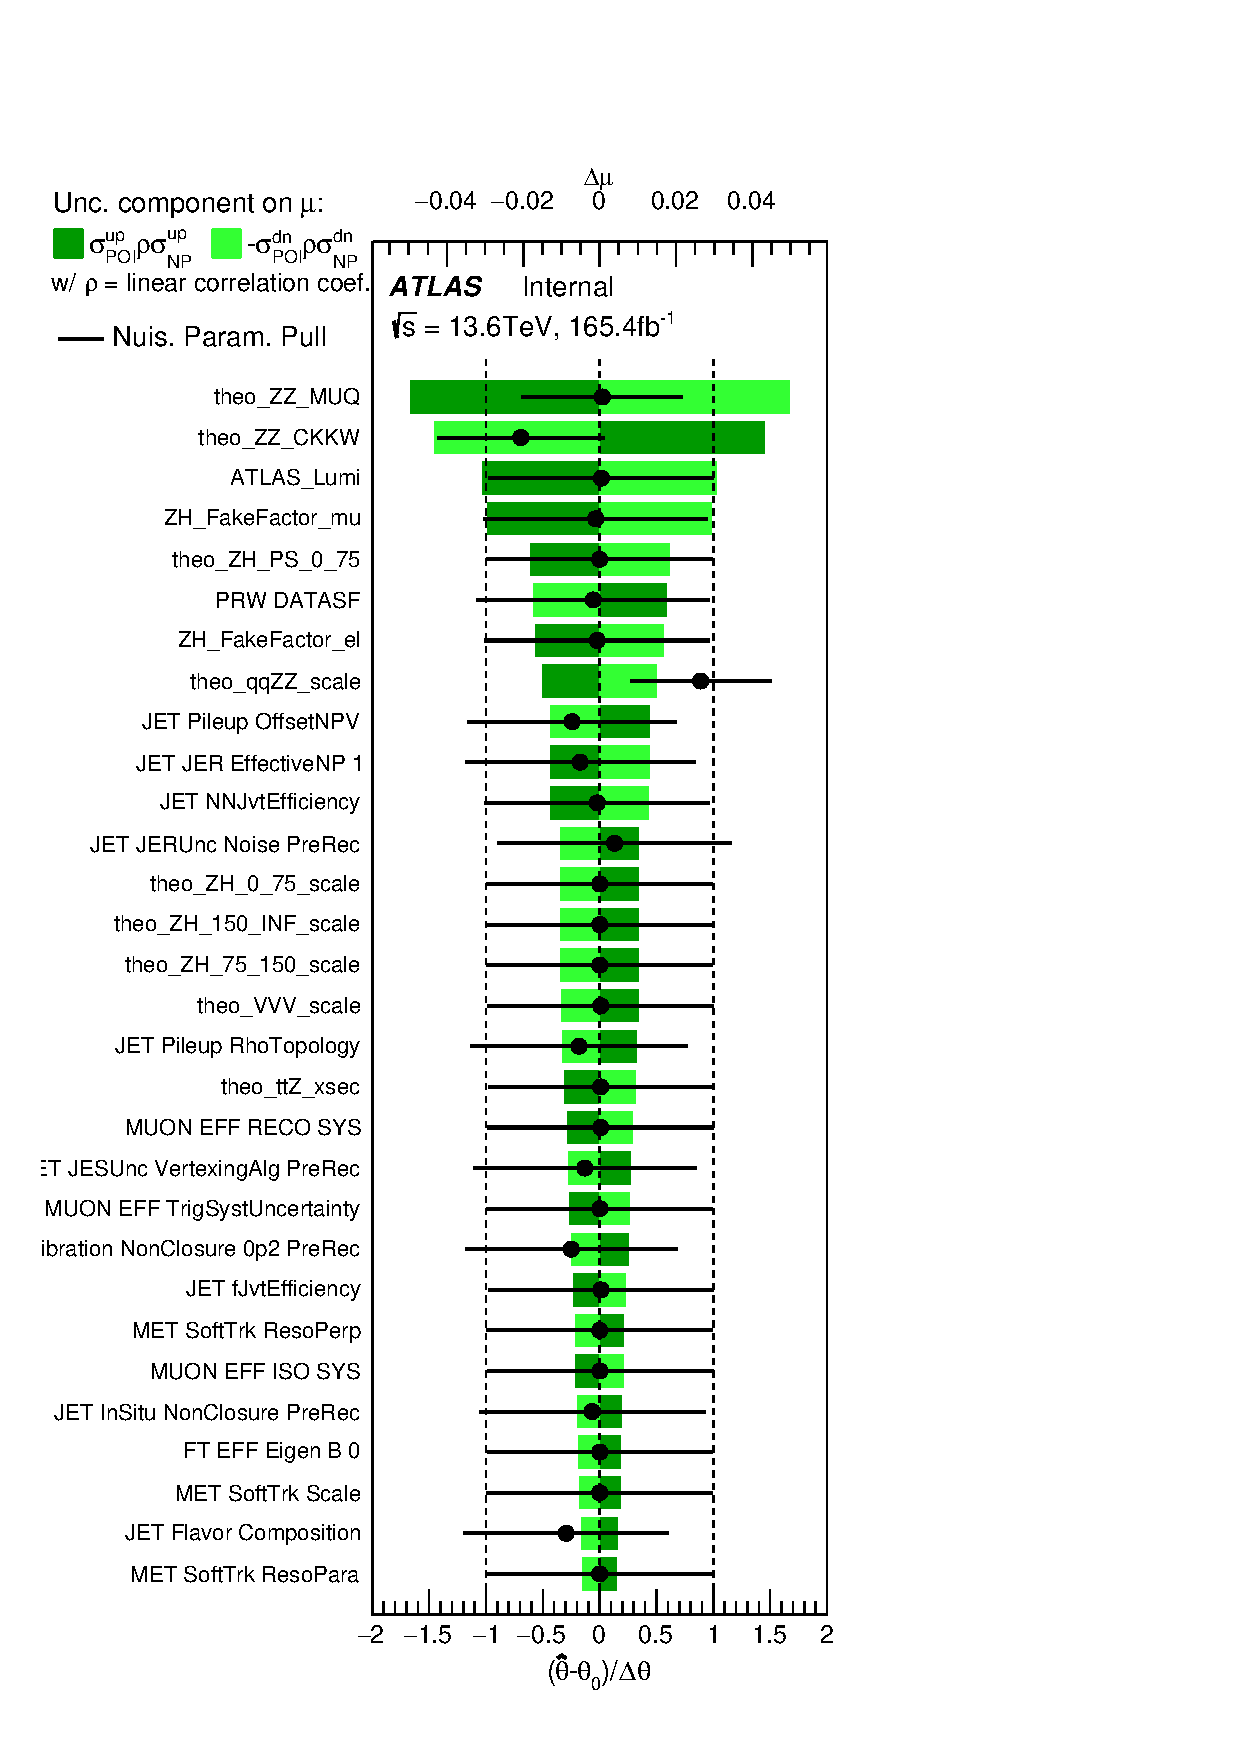
\includegraphics[width=0.3\linewidth]{figures/appendix/zh_stxs_results/rankings/Ranking_mu_ZH_0_75_Breakdown_stxs_1sfos.pdf}
    }
    \subfloat[Ranking: one SFOS $75 < \ptv{} < 150$~GeV.]{
        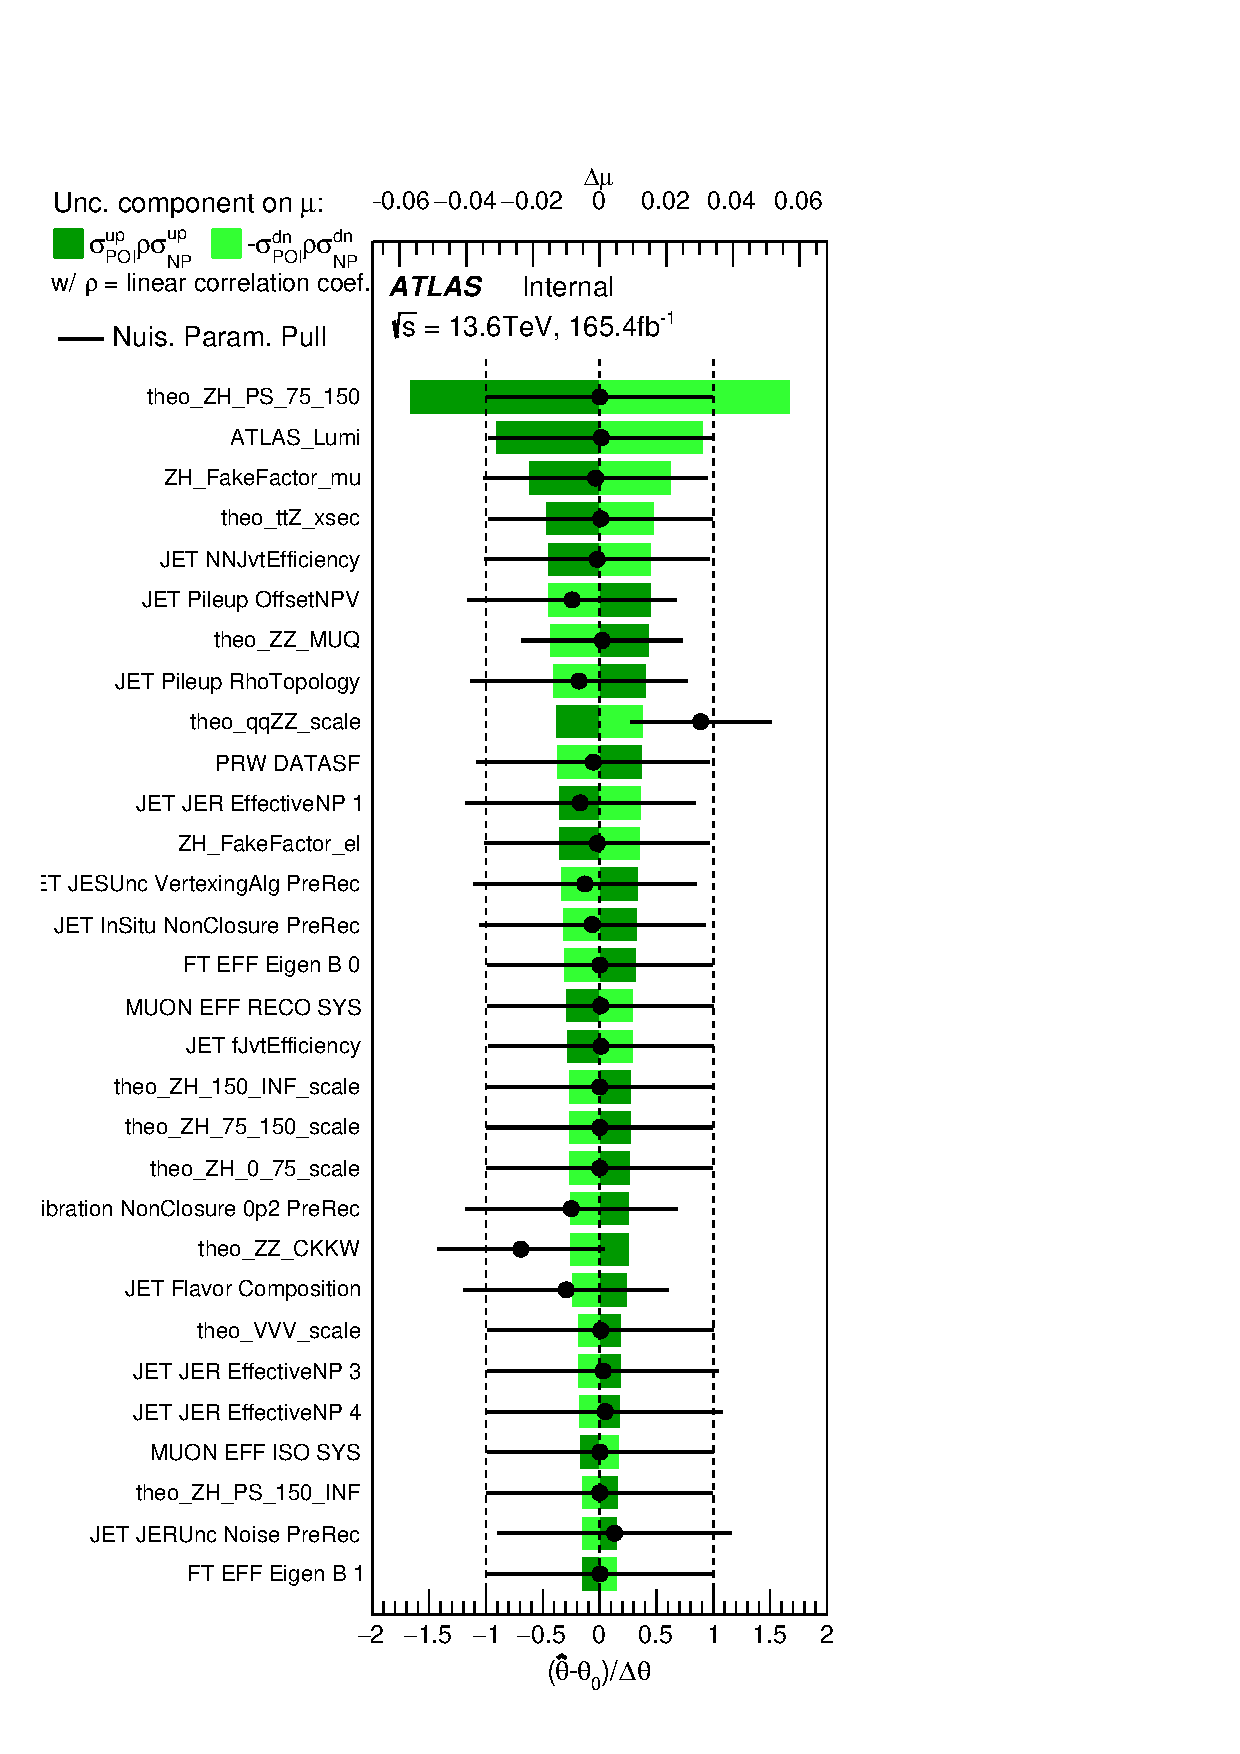
\includegraphics[width=0.3\linewidth]{figures/appendix/zh_stxs_results/rankings/Ranking_mu_ZH_75_150_Breakdown_stxs_1sfos.pdf}
    }
    \subfloat[Ranking: one SFOS $\ptv{} > 150$~GeV.]{
        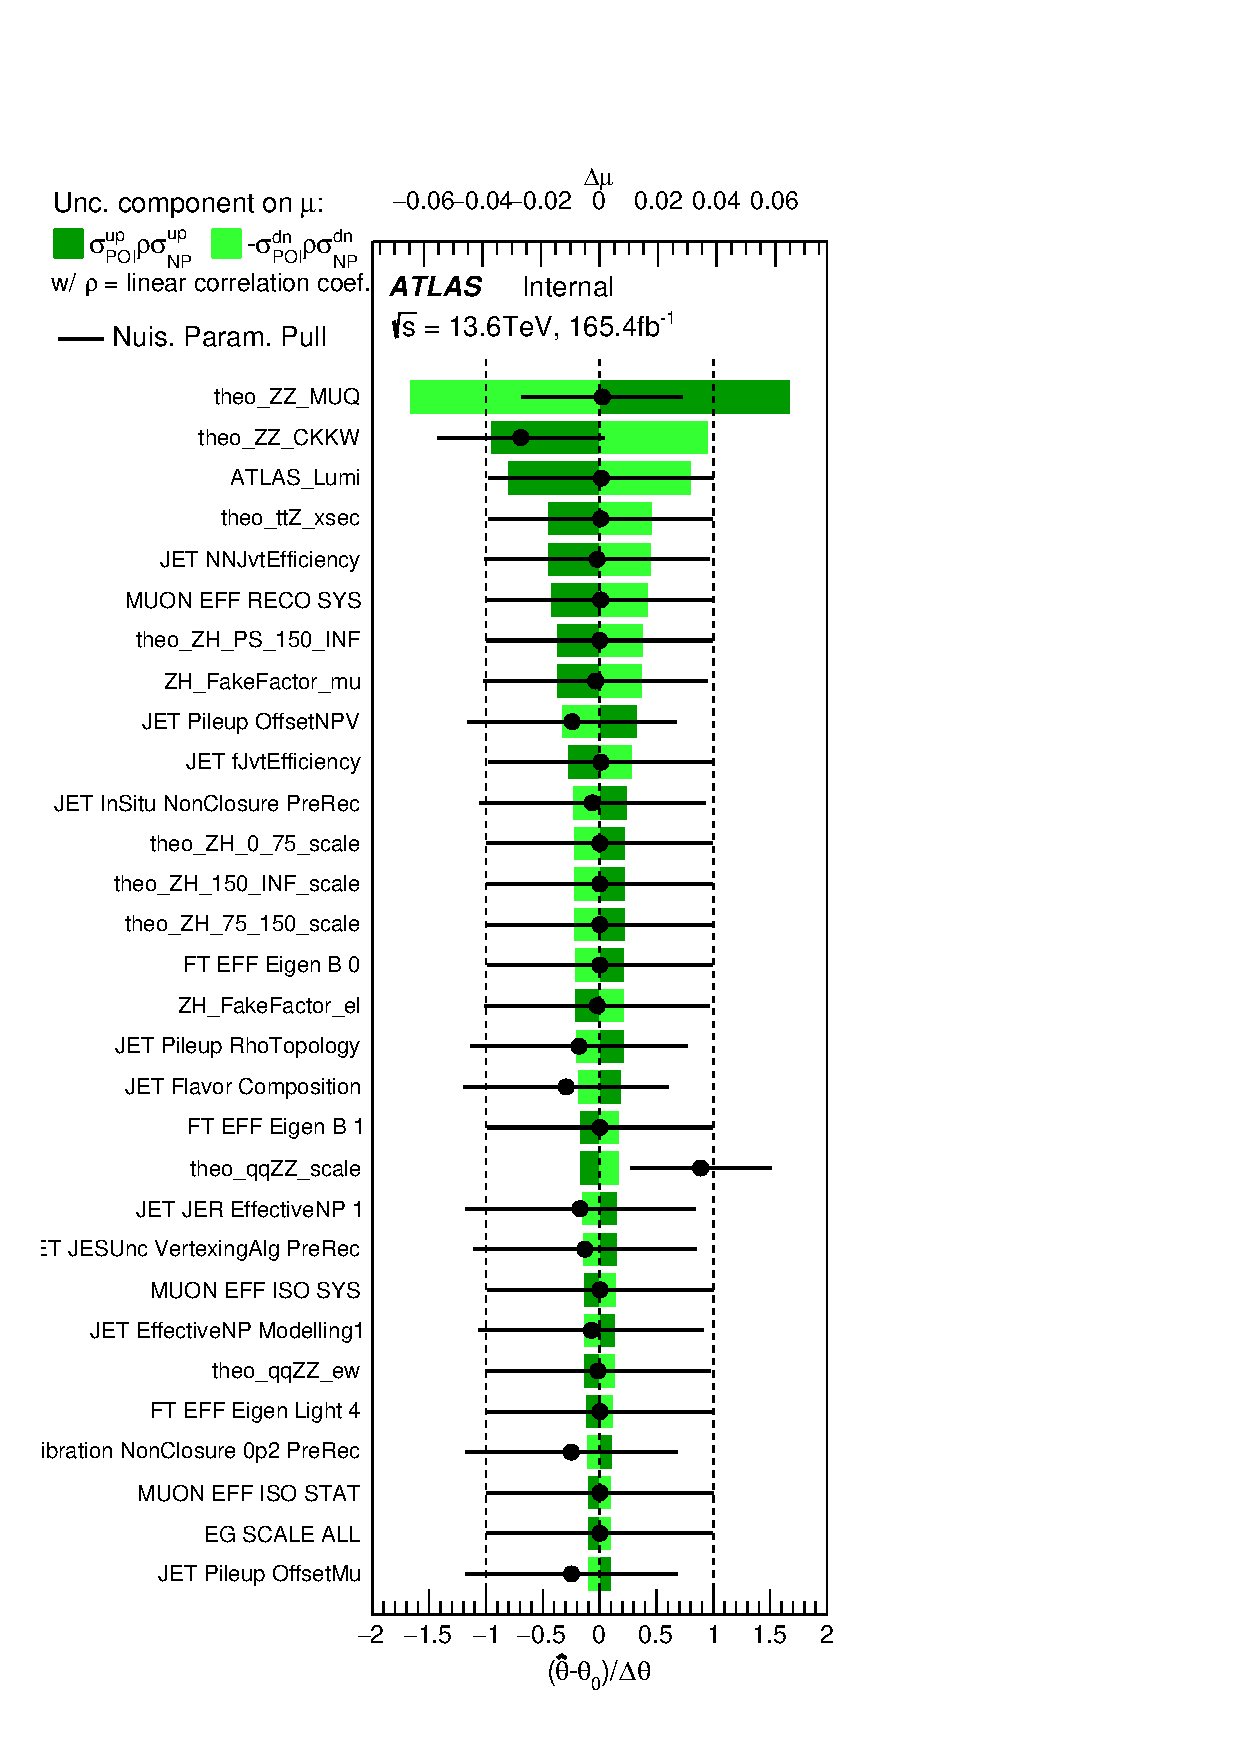
\includegraphics[width=0.3\linewidth]{figures/appendix/zh_stxs_results/rankings/Ranking_mu_ZH_150_inf_Breakdown_stxs_1sfos.pdf}
    }
    \caption{Systematic ranking plots for the one SFOS \zh{} STXS signal regions: (a) $0 < \ptv{} < 75$~GeV, (b) $75 < \ptv{} < 150$~GeV, and (c) $\ptv{} > 150$~GeV.}\label{fig:zh_stxs_ranking_plots_1sfos}
\end{figure}

\begin{figure}[htp]
    \centering
    \subfloat[Ranking: two SFOS $0 < \ptv{} < 75$~GeV.]{
        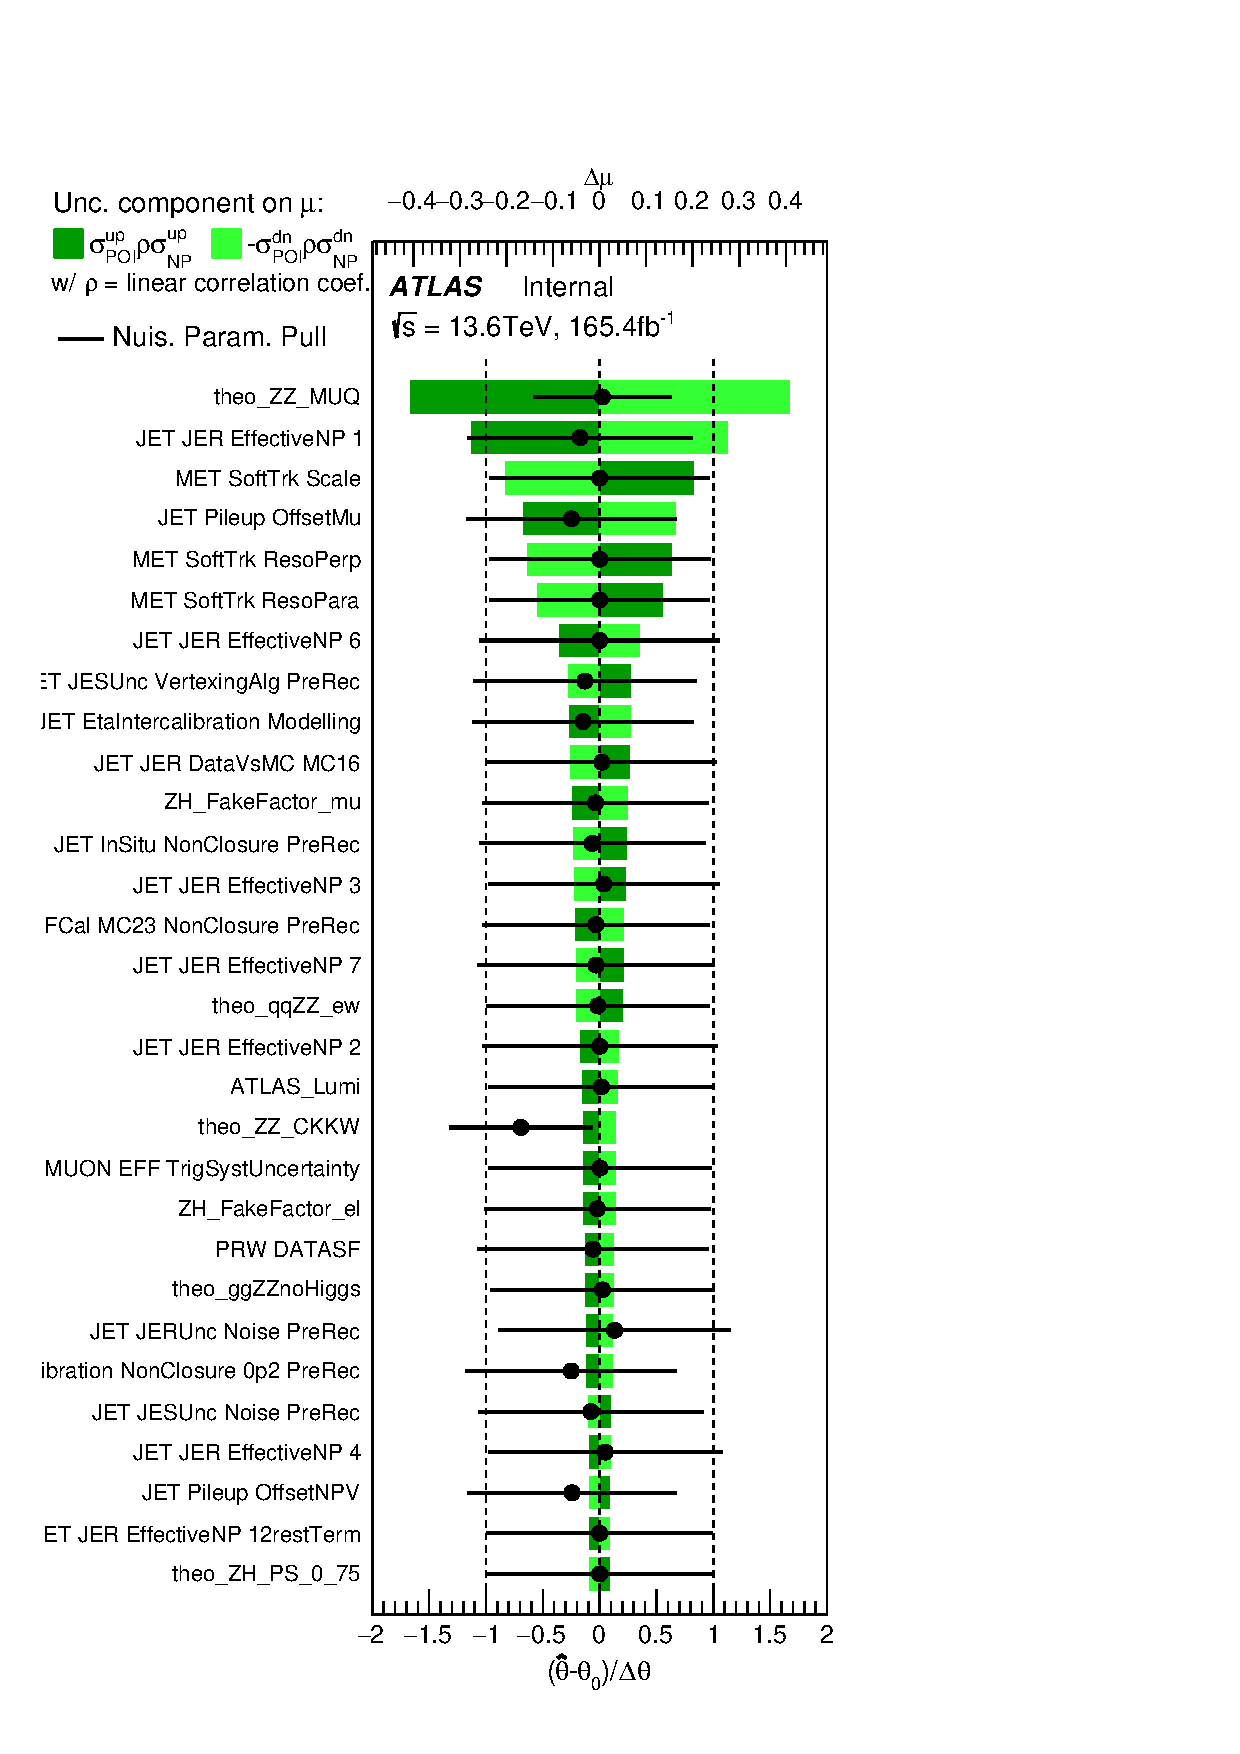
\includegraphics[width=0.3\linewidth]{figures/appendix/zh_stxs_results/rankings/Ranking_mu_ZH_0_75_Breakdown_stxs_2sfos.pdf}
    }
    \subfloat[Ranking: two SFOS $75 < \ptv{} < 150$~GeV.]{
        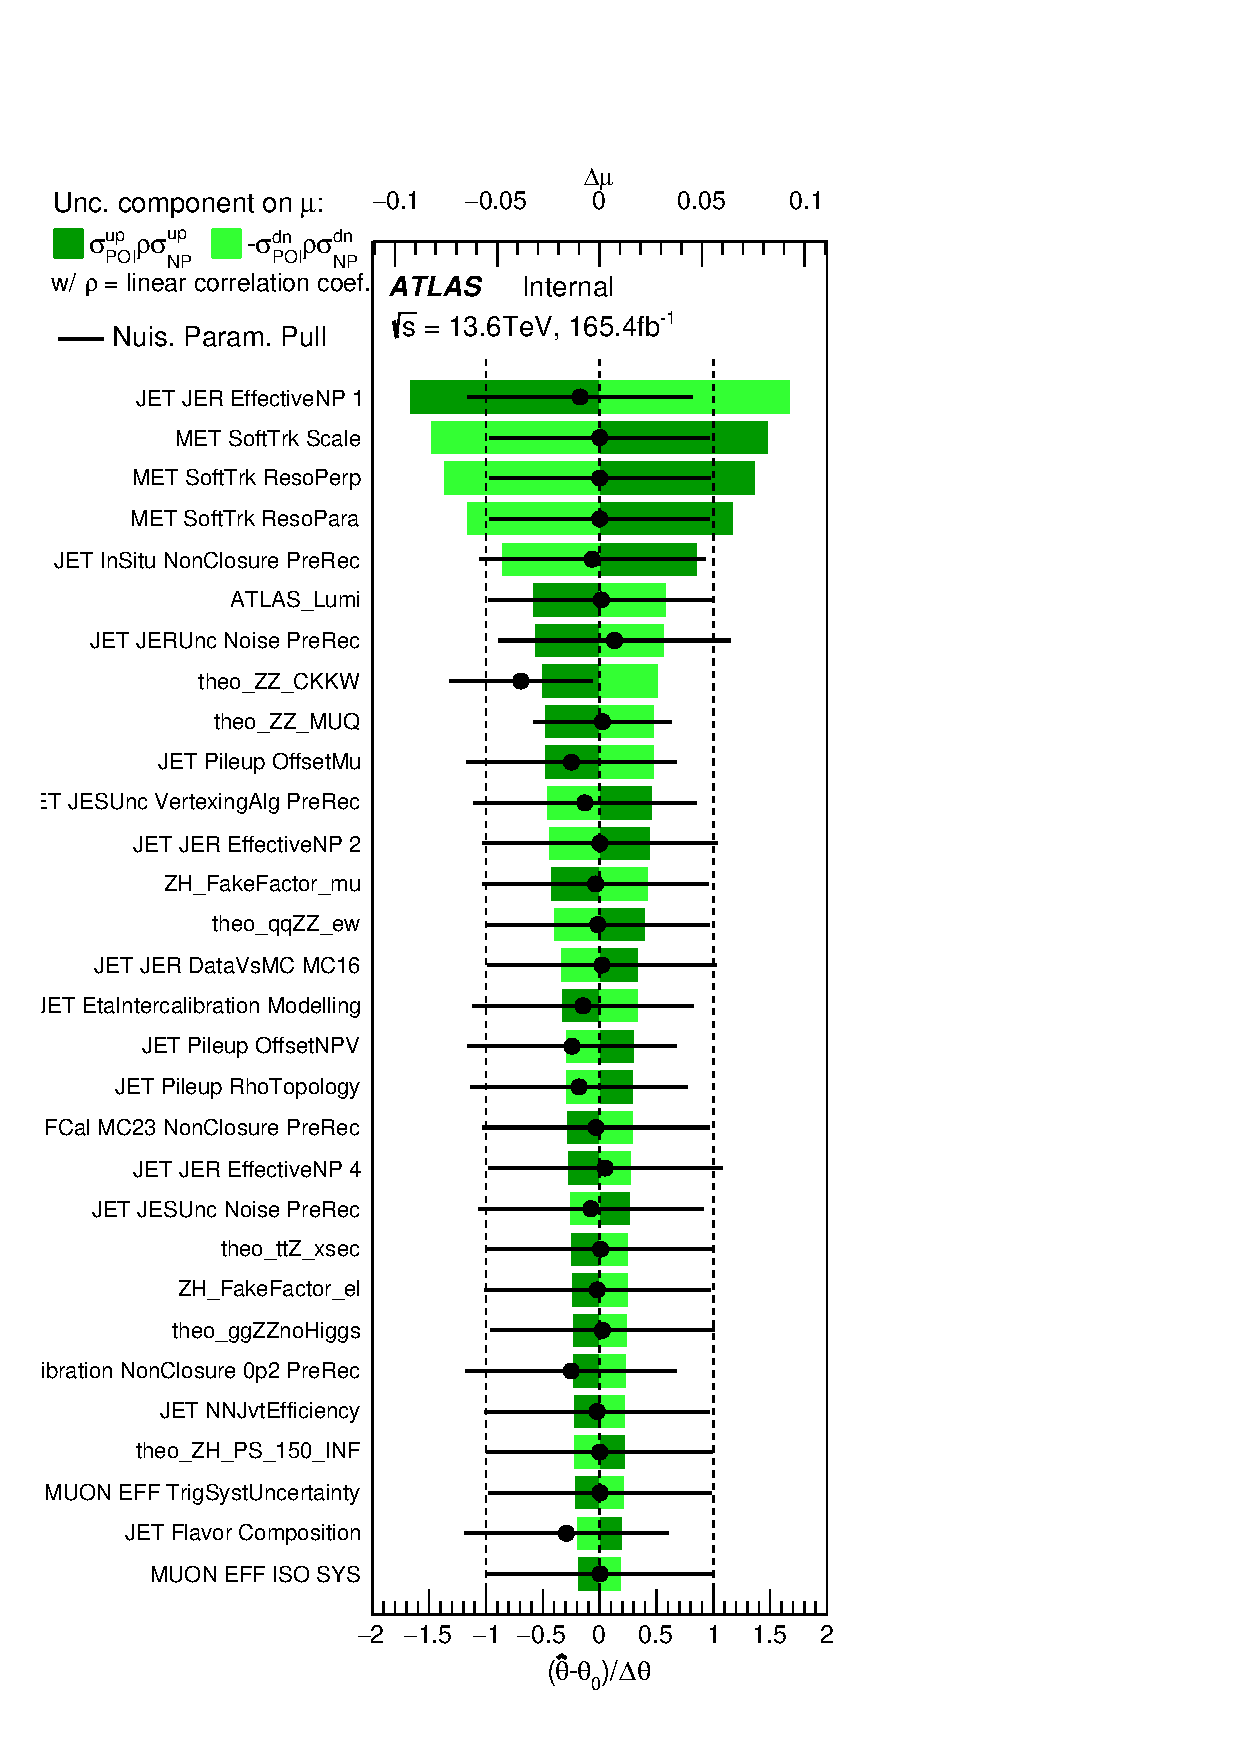
\includegraphics[width=0.3\linewidth]{figures/appendix/zh_stxs_results/rankings/Ranking_mu_ZH_75_150_Breakdown_stxs_2sfos.pdf}
    }
    \subfloat[Ranking: two SFOS $\ptv{} > 150$~GeV.]{
        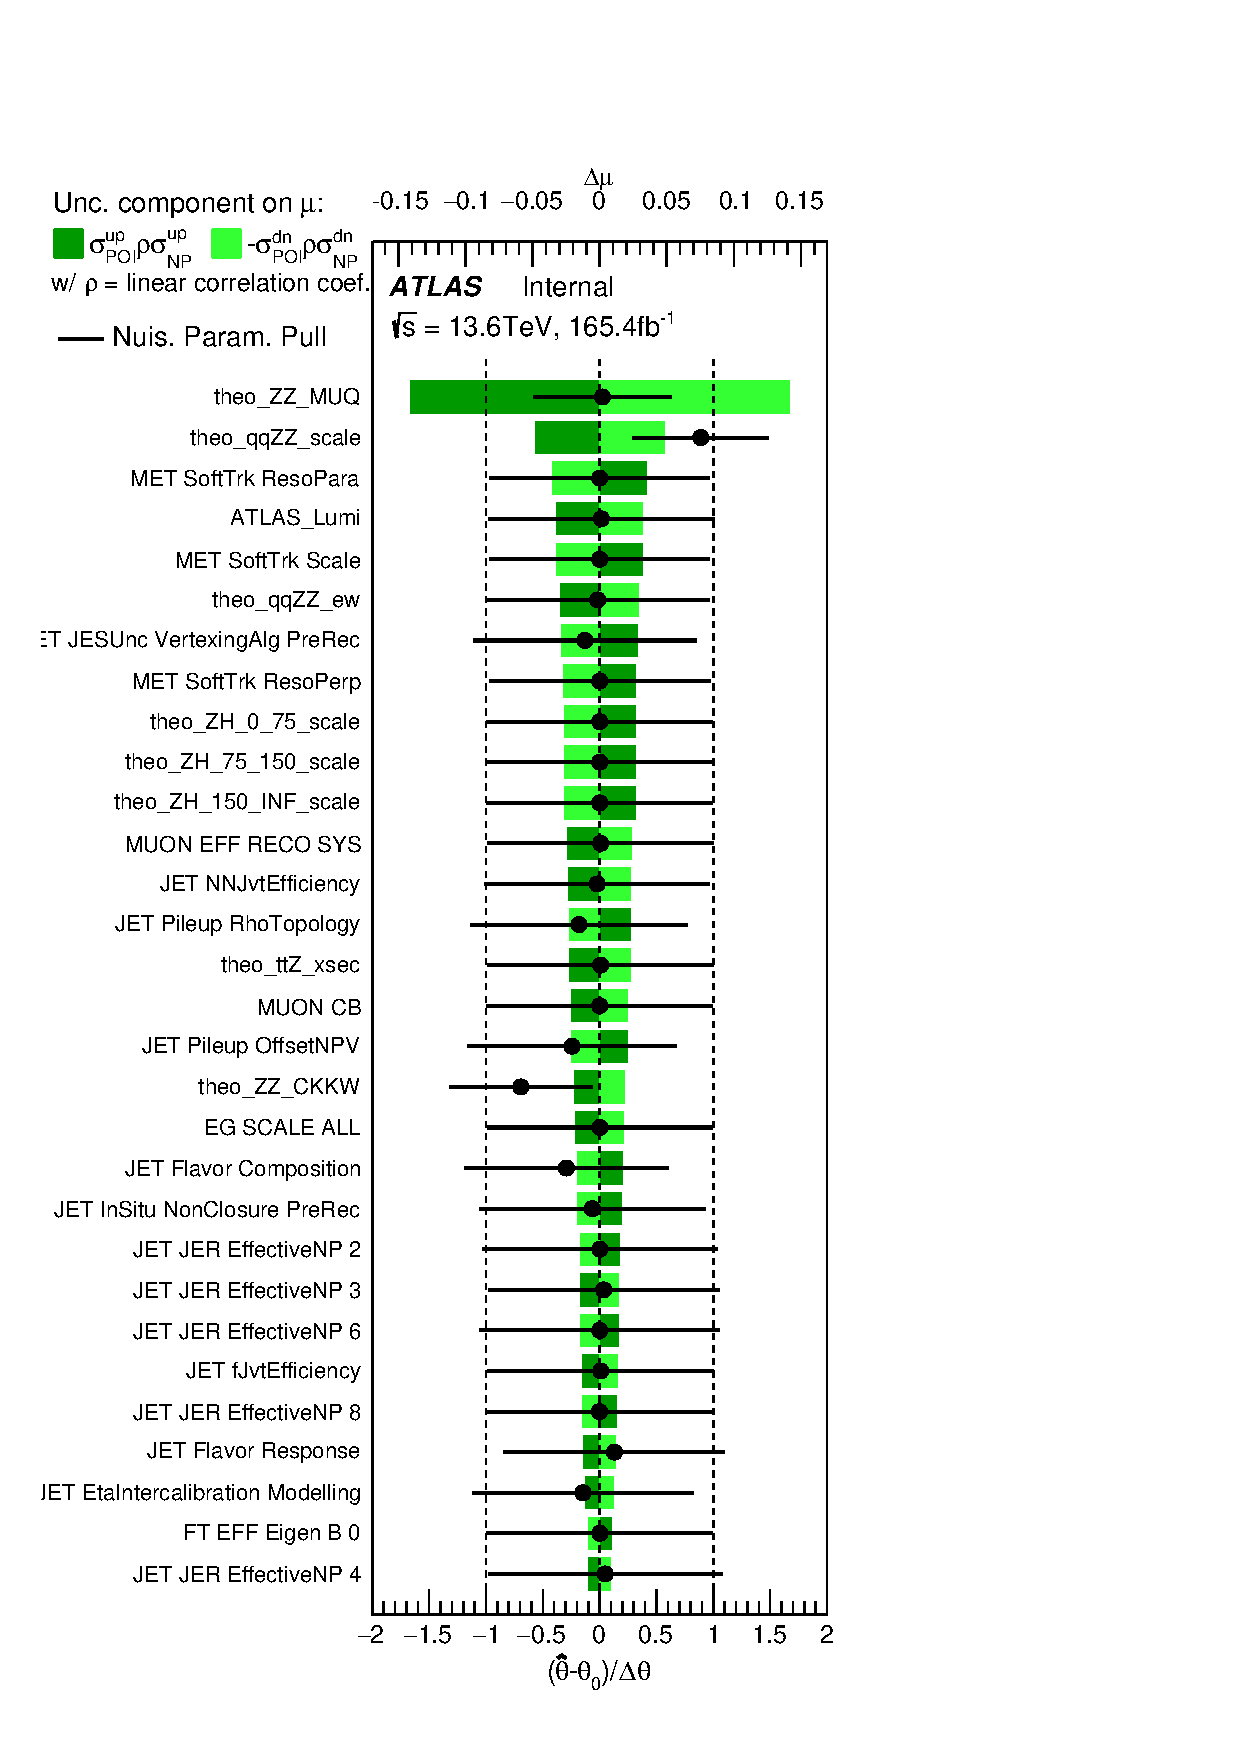
\includegraphics[width=0.3\linewidth]{figures/appendix/zh_stxs_results/rankings/Ranking_mu_ZH_150_inf_Breakdown_stxs_2sfos.pdf}
    }
    \caption{Systematic ranking plots for the two SFOS \zh{} STXS signal regions: (a) $0 < \ptv{} < 75$~GeV, (b) $75 < \ptv{} < 150$~GeV, and (c) $\ptv{} > 150$~GeV.}\label{fig:zh_stxs_ranking_plots_2sfos}
\end{figure}

\begin{figure}[htp]
    \centering
    \subfloat[Ranking: $0 < \ptv{} < 75$~GeV.]{
        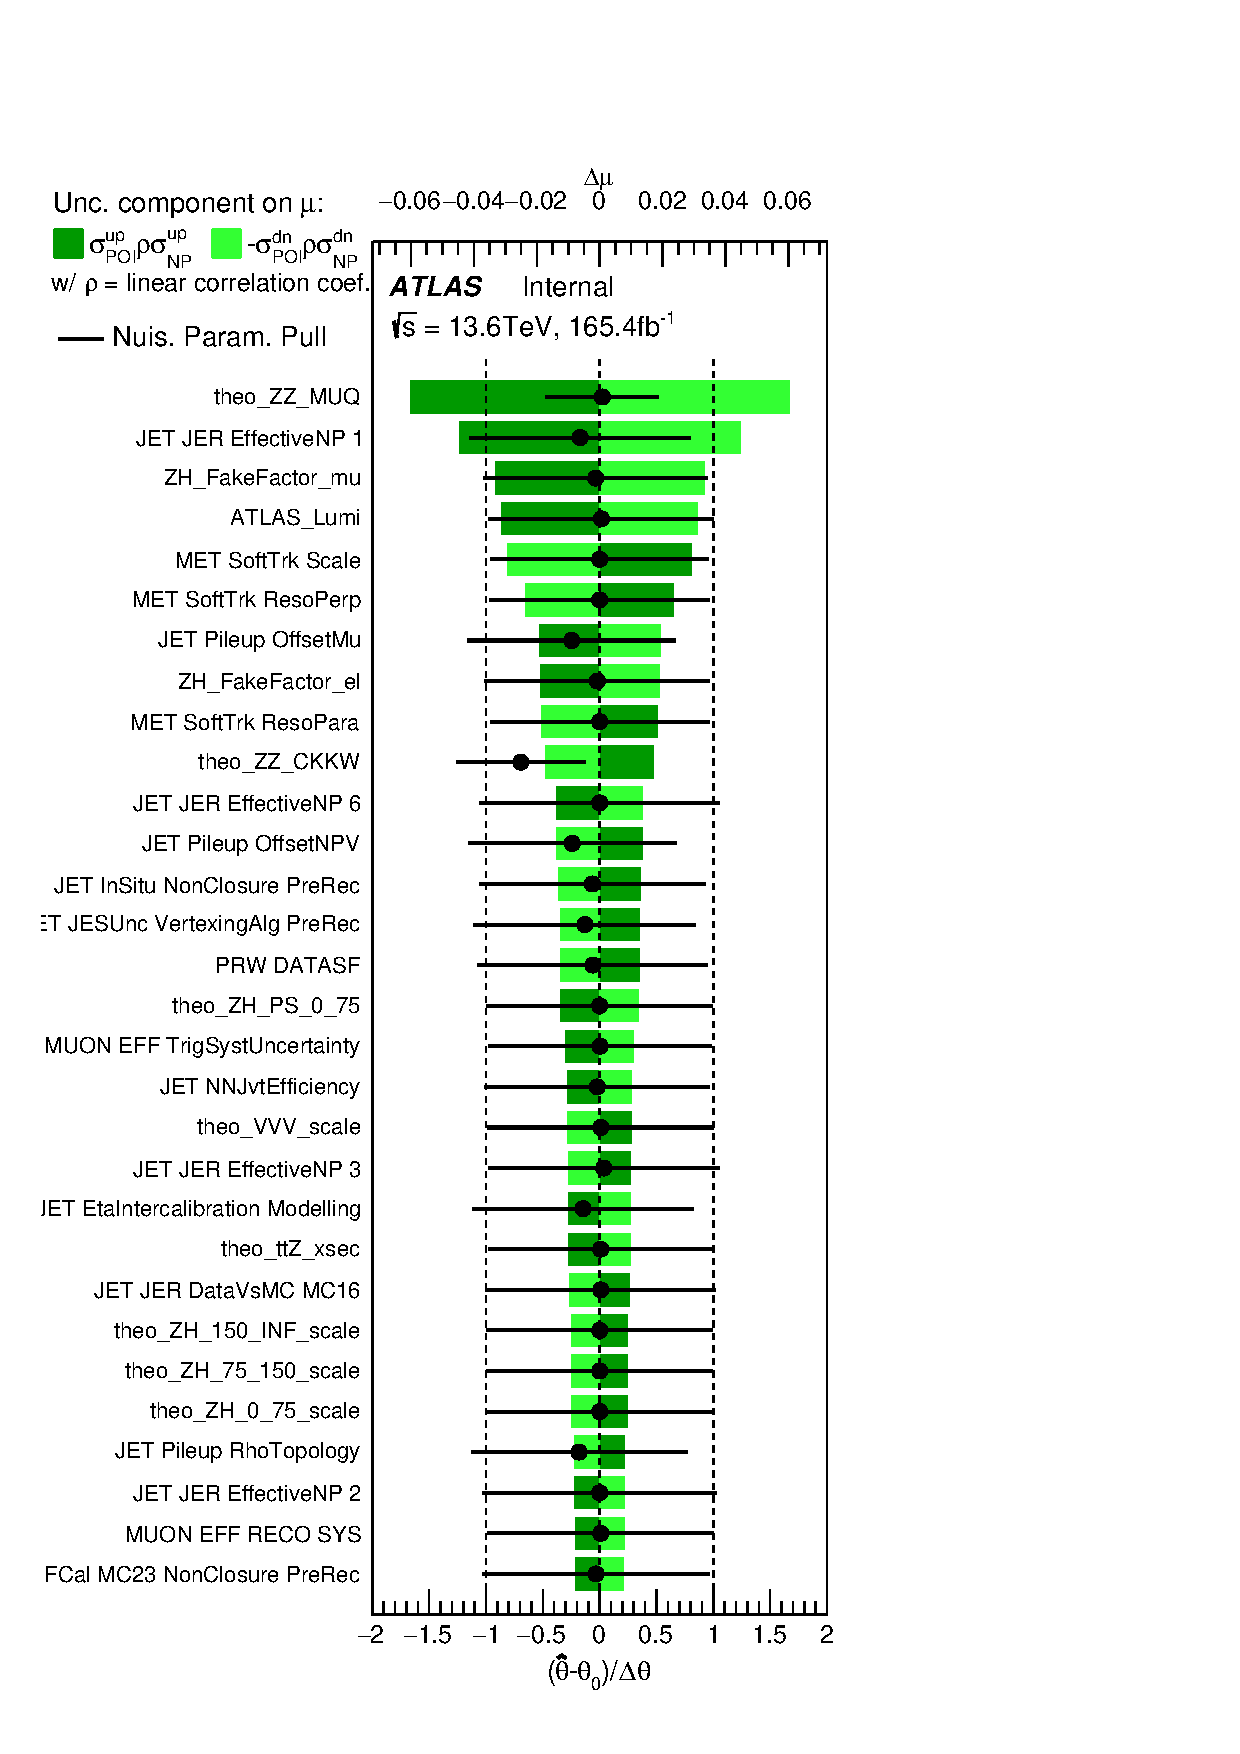
\includegraphics[width=0.3\linewidth]{figures/appendix/zh_stxs_results/rankings/Ranking_mu_ZH_0_75_Breakdown_stxs_combined.pdf}
    }
    \subfloat[Ranking: $75 < \ptv{} < 150$~GeV.]{
        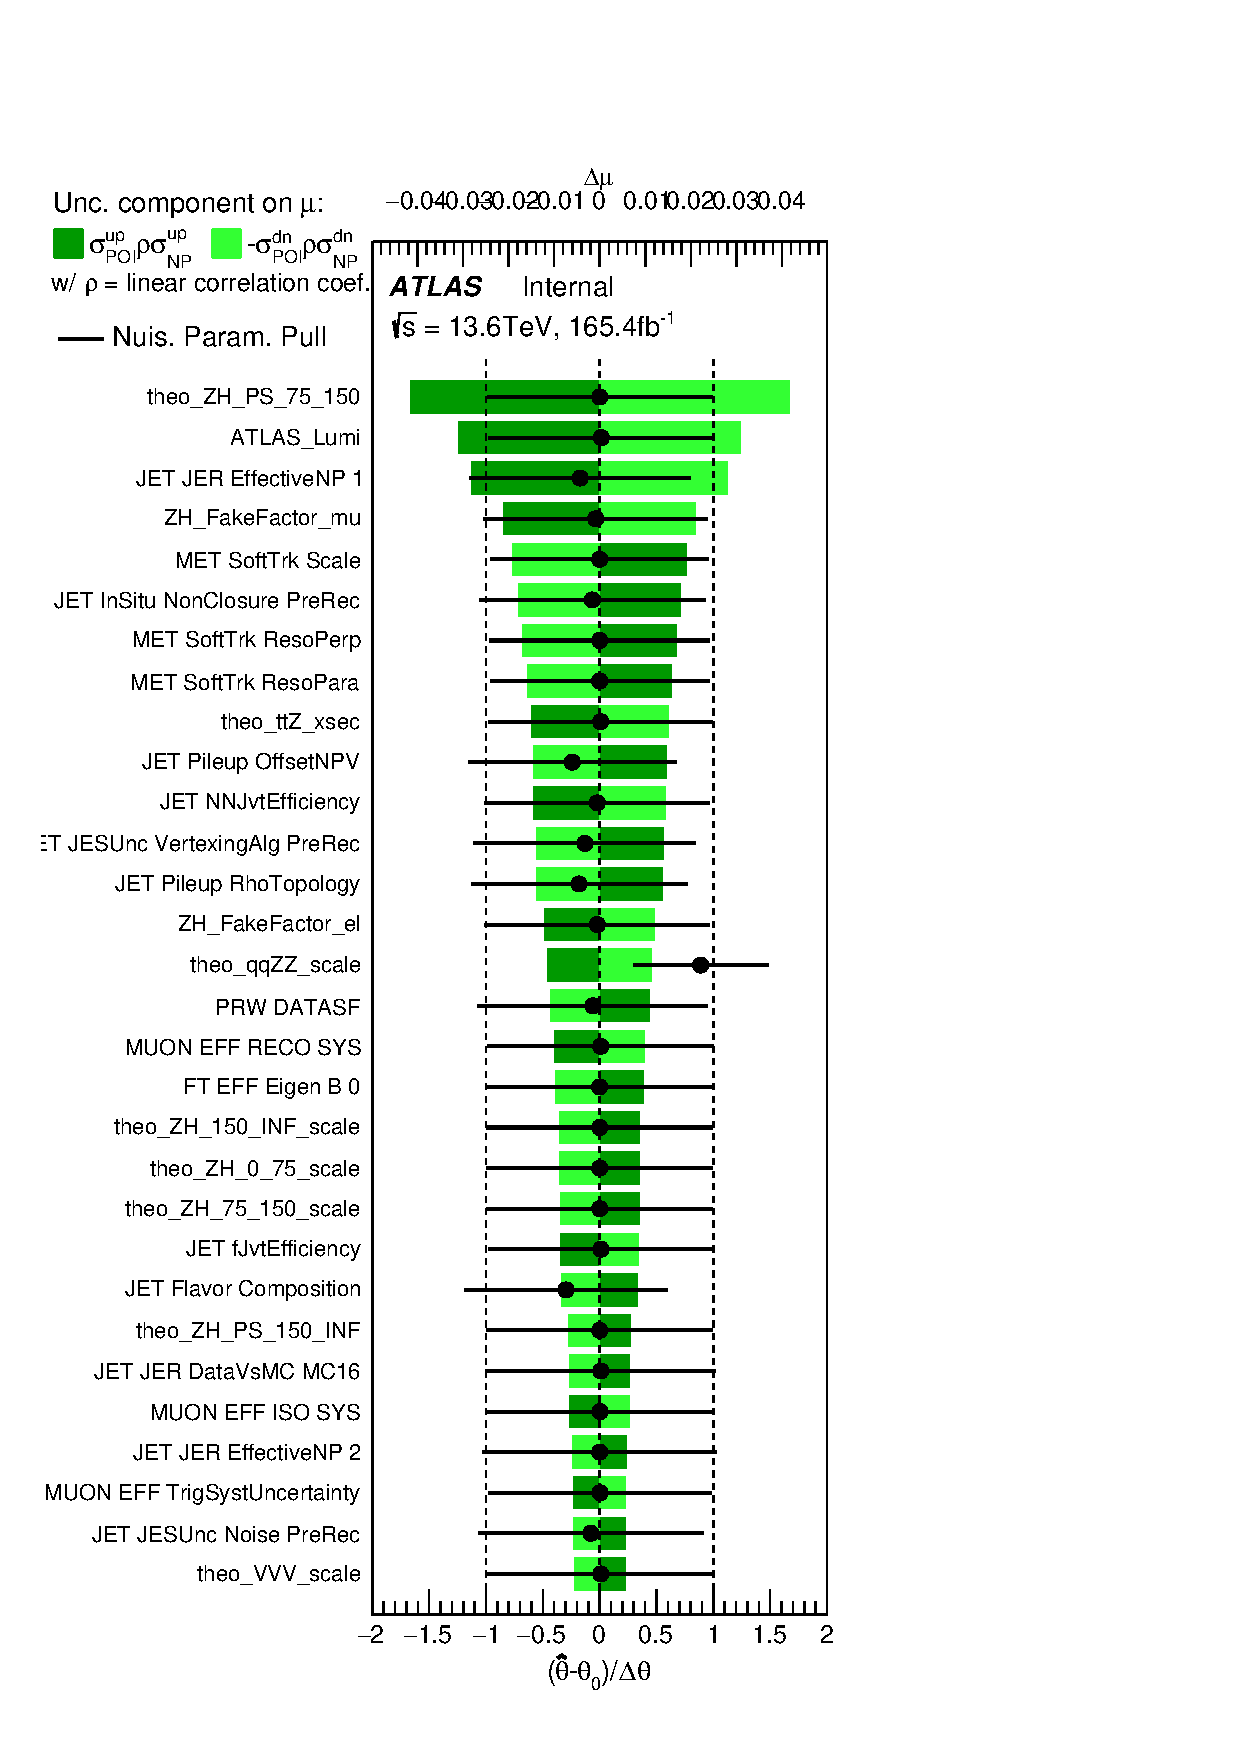
\includegraphics[width=0.3\linewidth]{figures/appendix/zh_stxs_results/rankings/Ranking_mu_ZH_75_150_Breakdown_stxs_combined.pdf}
    }
    \subfloat[Ranking: $\ptv{} > 150$~GeV.]{
        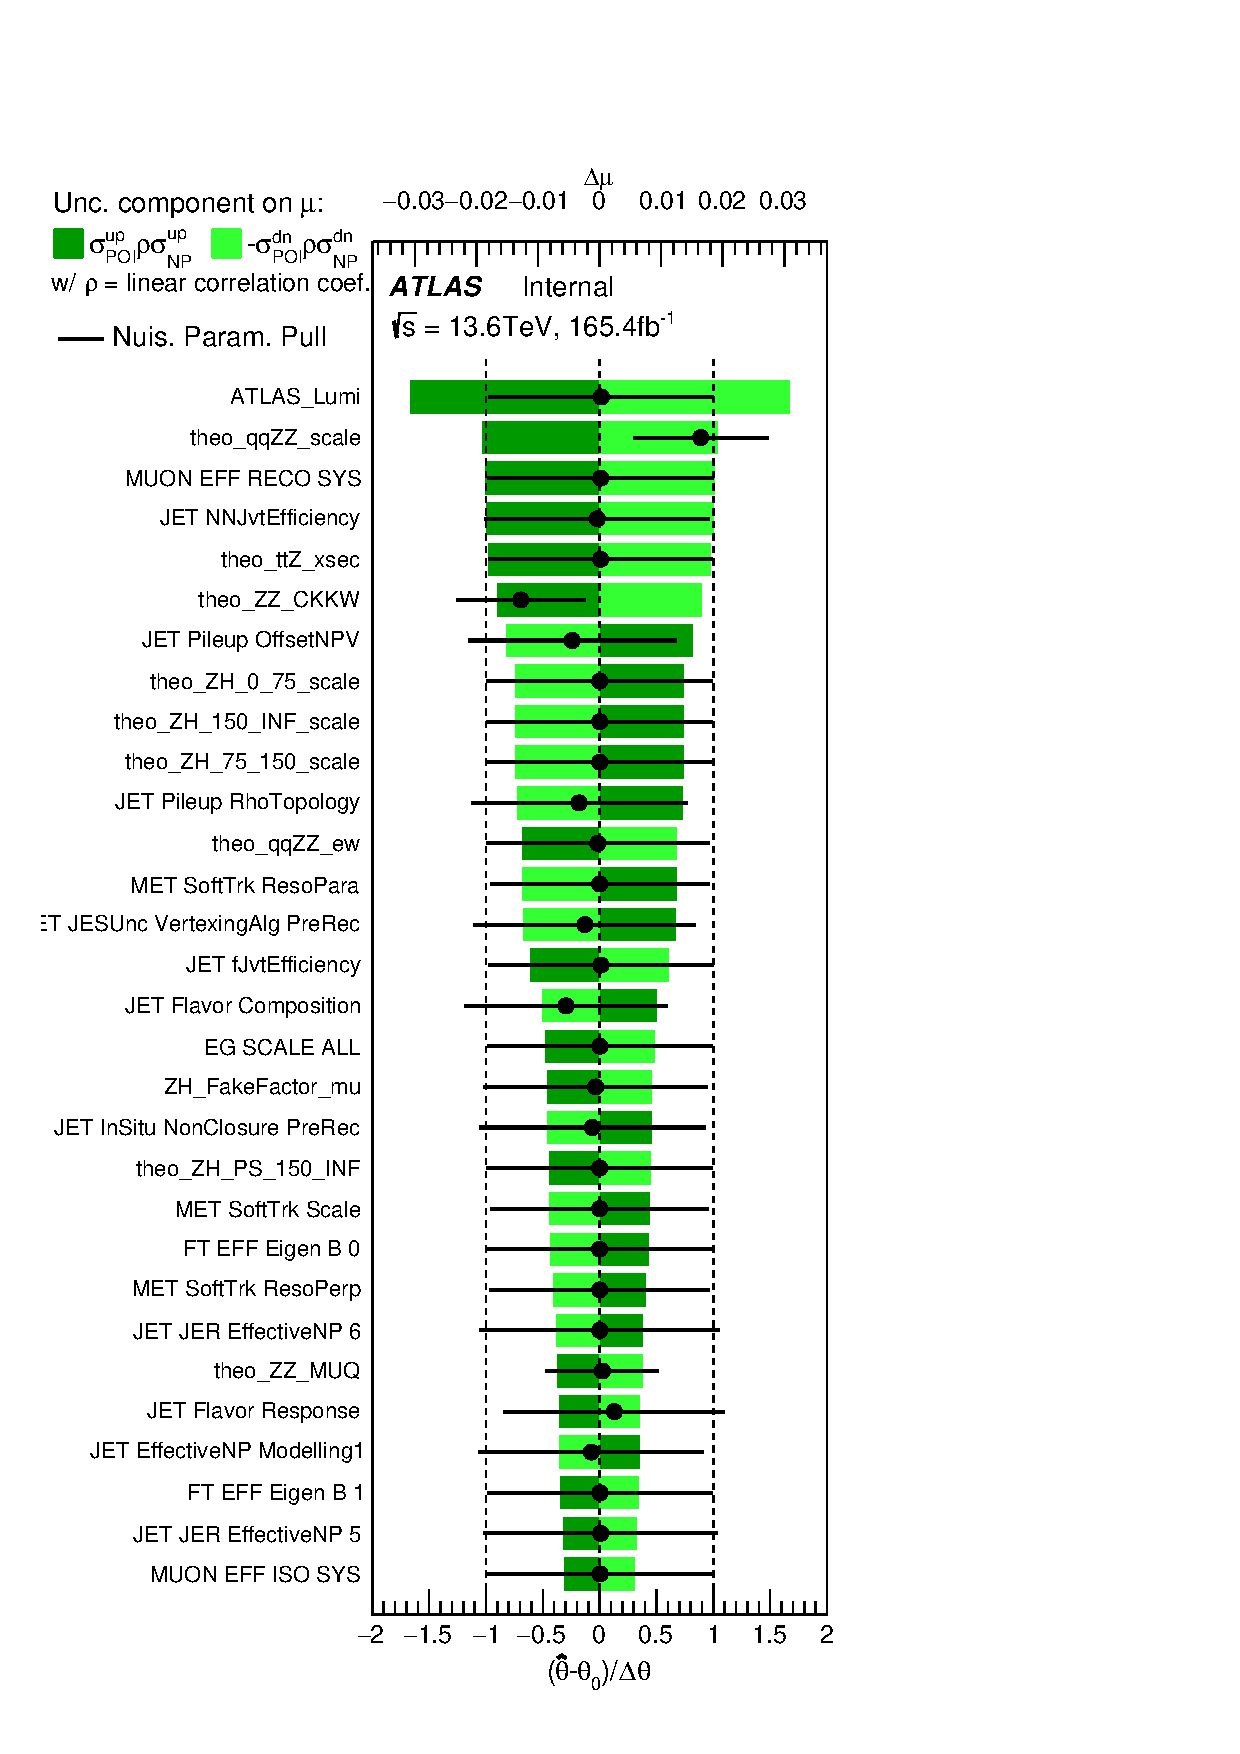
\includegraphics[width=0.3\linewidth]{figures/appendix/zh_stxs_results/rankings/Ranking_mu_ZH_150_inf_Breakdown_stxs_combined.pdf}
    }
    \caption{Systematic ranking plots for the combined \zh{} STXS signal regions: (a) $0 < \ptv{} < 75$~GeV, (b) $75 < \ptv{} < 150$~GeV, and (c) $\ptv{} > 150$~GeV.}\label{fig:zh_stxs_ranking_plots_combined}
\end{figure}
\clearpage{}